\section{Approach}
\label{section:approach}

\begin{figure}[t]
\begin{lstlisting}[frame=single,basicstyle=\ttfamily\small]	
void f()
{
    int x = g();
    if (x == VAL) {
        int y = x + 1;
        h(y);
    }
}
\end{lstlisting}
\vspace{-12pt}
\caption{Exemplary code sample.}
\label{figure:sample}
\end{figure}

\begin{figure*}[ht]
	\centering
	\begin{subfigure}[t]{0.33\textwidth}
		\centering
		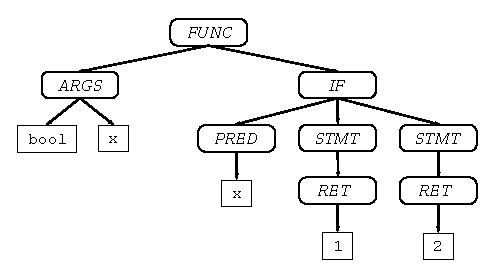
\includegraphics[width=1\textwidth,height=0.65\textwidth,keepaspectratio]{./figure/ast.eps}
		\caption{Abstract Syntax Tree}
		\label{figure:ast}
	\end{subfigure}
	\begin{subfigure}[t]{0.33\textwidth}
		\centering
		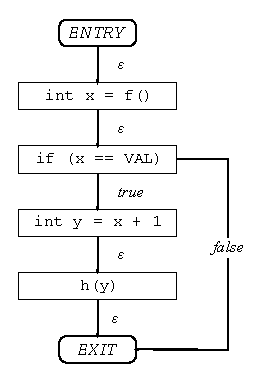
\includegraphics[width=2\textwidth,height=0.65\textwidth,keepaspectratio]{./figure/cfg.eps}
		\caption{Control Flow Graph}
		\label{figure:cfg}
	\end{subfigure}
	\begin{subfigure}[t]{0.33\textwidth}
		\centering
		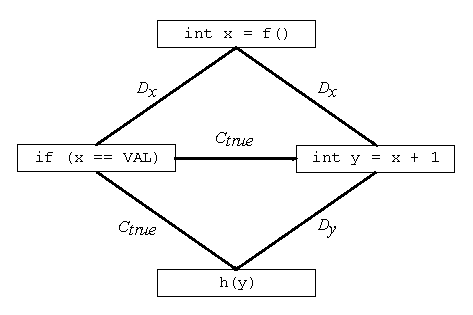
\includegraphics[width=1\textwidth,height=0.65\textwidth,keepaspectratio]{./figure/pdg.eps}
		\caption{Program Dependency Graph}
		\label{figure:pdg}
	\end{subfigure}
	\caption{Representations of code for the example in Figure~\ref{figure:sample}.}
\end{figure*}

\begin{figure*}[ht]
	\centering
	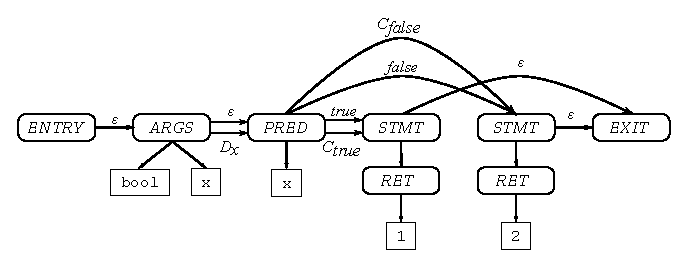
\includegraphics[width=0.7\textwidth,height=0.65\textwidth,keepaspectratio]{./figure/cpg.eps}
	\caption{Code Property Graph}
	\label{figure:cpg}
\end{figure*}

To address the limitations identified in the previous section, we need representation more comprehensive than those used in existing vulnerability detection methods.
Execution time of detection should also be scalable.
Deep learning can achieve both effectiveness and efficiency of detection.
Shin et al. found that applying deep learning for software analysis has advantages in many perspectives \cite{shin2015recognizing}.
To use deep learning, how to represent input data and learning model should be decided.

The way of representing dataset, i.e. softwares, should meet the following criteria:

\textbf{Representation Granularity.}
Each element of representation should include information of software in order to achieve function-level granularity.
Representation should be able to determine in which function the vulnerability resides, which cannot be accomplished with simple code metrics such as LoC.
Therefore, information of software should be distributed to detailed component of program structure to help model determine the exact location of vulnerability.
Both the raw form such as binary \cite{shin2015recognizing, kosmidis2017machine} and preprocessed form such as abstract syntax trees \cite{wang2016automatically}
have been used as representation of software for deep learning models.

\textbf{Program Context.}
Since same code can be either safe or vulnerable depending on the context,
detailed information of control flow and dependence of program are also required.
This difference is, although inherent, not distinguished explicitly by program structures only.
Hence, such information should also be shown in representation.

\subsection{Representation}
I use code property graph to satisfy requirements described above.
Code property graph was introduced to effectively mine large amounts of source code for vulnerabilities \cite{yamaguchi2014modeling}.
Code property graph combines abstract syntax tree, control flow graph and program dependency graph.
Thus, syntactic structure, control flow and dependency between each part of software code are included, successfully meeting requirements mentioned above.

\textbf{Abstract Syntax Tree (AST)}
Abstract syntax trees represent structure of source code in an abstract way.
Figure~\subref{figure:ast} shows example AST for the code sample Figure~\ref{figure:sample}.
Their nodes do not necessarily correspond to exact syntax token of the program but can represent larger semantic unit such as condition expression or variable declaration.

\textbf{Control Flow Graph (CFG)}
Control flow graph describes conditions and order of each execution path of program.
Figure~\subref{figure:cfg} shows example CFG for the code sample given above.
While control flow graph provides information of condition and context, data flow is still required to determine the exact attack vector.

\textbf{Program Dependency Graph (PDG)}
Program dependency graph consists of two types of edges: data dependency edges and control dependency edges.
Figure~\subref{figure:pdg} shows example PDG for the code sample given above, data and control dependency edges are labeled as D and C respectively.
Data dependency edges connect variable values and statements affected by them.
Control dependency edges are different from control flow graph since the former do not contain execution order but show dependencies more clearly.

The combination of three graphs forms code property graph shown in Figure~\ref{figure:cpg}.

\subsection{Learning Model for Graph Data}

Since we use code property graph as program representation, we need neural network model which takes graph data as input.
Code property graph is a directed multigraph with edges containing multiple, isolated attributes.
We consider typical learning models for graph data:

\textbf{Support Vector Machine with Graph Kernel.}
Support vector machine (SVM) is a type of machine learning that can classify input data.
SVM calculates decision surface using cross products of inputs.
Although SVM is not deep learning method, it can be used as baseline.
Kernel in SVM is a function that adjusts input data or their cross products.
Kernel is used to help SVM to classify data more efficiently, by mapping different inputs more distinctly.
Graph kernel, a kernel function for graph input, has been mainly applied in bioinformatics and cheminformatics, for instance, predicting protein function by its structure.
Classical graph kernels are based on walks, paths, subgraphs or subtrees.

Weisfeiler-Lehman (WL) graph kernel \cite{shervashidze2011weisfeiler} is state-of-the-art among graph kernels.
WL graph kernel generates feature vector from subtree pattern in every iteration.
In algorithm, neighborhood information is compressed to label of each node.
Feature vector are then created in each iteration, consists of numbers of each label appeared during the algorithm.
The similarity between graphs are calculated as the inner product of their feature vectors.

\textbf{Graph Neural Network.}
Graph neural network (GNN) is a learning model which directly uses input graph layout as model \cite{gori2005new}.
GNN extends recursive neural networks, using nodes of input graph as state representations.
For each iteration, state values are updated by being propagating by other connected states.
GNN eventually generates some desired attribute of the input graph.
Li et al. introduced Gated graph sequence neural network (GGS-NN) based on GNN.
GGS-NN is an extended	 model of GNN which can find the output sequence of graph producing such attribute \cite{li2015gated}.

\textbf{Convolutional Neural Network for Graph.}
Niepert et al. presented an approach to process general graphs with CNN by considering input of classical CNN as lattice graph \cite{niepert2016learning}.
From such perspective, receptive field of classical CNN is a neighborhood subgraph from certain node with fixed width.
Thus for an arbitrary input graph, receptive field can be generated and consequently passed as input to classical CNN.